\section[Limiten und Kolimiten]{Limiten und Kolimiten \hfill \small
Kathrin Gimmi}

\emph{Werbung:} Wir verstehen, was allgemeine Limiten und Kolimiten von
Diagrammen sind. Dazu wird es viele Beispiele geben, unter anderem die uns
schon bekannten Produkte und Koprodukte. Speziell sind sog. filtrierte
Kolimiten wichtig, da diese in der täglichen Praxis oft vorkommen und besonders
schöne Eigenschaften haben. Abschließend werden wir die Frage diskutieren, wie
man Kategorien, denen es an Limiten oder Kolimiten mangelt, vervollständigen
kann.

In diesem Abschnitt wollen wir Funktoren~$\I \to \C$ auch als~($\I$-förmige)
Diagramme bezeichnen.


\subsection{(Ko-)Kegel und (Ko-)Limiten}

\begin{defn}Ein \emph{Kegel} eines Diagramms~$F : \I \to \C$ besteht aus
\begin{enumerate}
\item einem Objekt~$K \in \Ob \C$ (der sog. \emph{Kegelspitze}) zusammen mit
\item jeweils einem Morphismus~$\pi_i : K \to F(i)$ für jedes Objekt~$i \in \Ob\I$,
\end{enumerate}
sodass
für alle Morphismen~$f : i \to j$ in~$\I$ die Dreiecke
\[ \xymatrix{
  & K \ar[ld]_{\pi_i} \ar[rd]^{\pi_j} \\
  F(i) \ar[rr]_{F(f)} && F(j)
} \]
kommutieren.
\end{defn}
Die Notation etwas missbrauchend werden Kegel oft nur nach ihrer Kegelspitze
genannt, obwohl die Morphismen~$\pi_i$ mit zum Datum gehören.
Die Morphismen~$\pi_i$ werden manchmal als Projektionsmorphismen
bezeichnet, der Grund dafür wird beim ersten Beispiel klar werden.

\begin{defn}Ein \emph{Morphismus von Kegeln $K \to \widetilde K$} eines Diagramms~$F$ besteht aus
\begin{enumerate}
\item[] einem Morphismus der Kegelspitzen $\psi : K \to \widetilde K$ in~$\C$
\end{enumerate}
sodass
\begin{enumerate}
\item[]
für alle~$i \in \Ob\I$ die Dreiecke
\[ \xymatrix{
  K \ar[rr]^{\psi} \ar[rd]_{\pi_i} && \widetilde K \ar[ld]^{\widetilde\pi_i} \\
  & F(i)
} \]
kommutieren.
\end{enumerate}
\end{defn}
Abbildung~\ref{kegel} erklärt die Herkunft des Begriffs "`Kegel"'.

\begin{figure}
  \[
    \xymatrix{
      K \ar@[grey]@{-->}[rrrrr]
      \ar@[grey][dddr] \ar@[grey][dddrrr] \ar@[grey][dddrrrr] \ar@[grey][ddddrr] &&&&&
      \widetilde K \ar@[grey][dddl] \ar@[grey][dddll] \ar@[grey][dddllll]
      \ar@[grey][ddddlll]
      \\\\\\
      & F(i) \ar[rr] \ar[rd] && F(j) \ar[r] \ar[ld] & F(\ell) \\
      & & F(k)
    }
  \]
  \caption{\label{kegel}Zwei Kegel und ein Kegelmorphismus zwischen ihnen.}
\end{figure}

Kegelmorphismen kann man auf die offensichtliche Art und Weise miteinander
verketten (einfach die Morphismen der Kegelspitzen verketten). Daher ist es
sinnvoll, von der \emph{Kategorie der Kegel} zu einem festen
Diagramm~$F:\I\to\C$ zu sprechen. Terminale Objekte dieser Kategorie haben
einen besonderen Namen:
\begin{defn}Ein \emph{Limes} eines Diagramms~$F:\I\to\C$ ist ein terminales
Objekt in der Kategorie der Kegel zu~$F$.\end{defn}
Da allgemein terminale Objekte einer Kategorie bis auf eindeutige Isomorphie
eindeutig sind (siehe Aufgabe~2 von Übungsblatt~2), folgt sofort folgende
Beobachtung:
\begin{prop}Limiten sind bis auf eindeutige Isomorphie eindeutig. Die
Kegelspitzen von Limiten sind zumindest bis auf Isomorphie eindeutig.\end{prop}

Für ein anschauliches Verständnis von Limiten sind zwei Mottos wichtig:
\begin{motto}Ein Limes eines Diagramms ist ein bestes
(größtmögliches) Objekt, welches das Diagramm zu einem Kegel ergänzt.
\end{motto}
\emph{Größtmöglich} ist dabei nicht im wörtlichen Sinn, wie er etwa in der Kategorie
der Mengen vorstellbar ist, zu interpretieren, sondern nur so zu verstehen,
als dass jeder andere Kegel
(Möchtegern-Limes) einen Morphismus in den Limes hinein besitzt.

\begin{motto}\label{limessubsumiert}
Ein Limes subsumiert das gesamte Diagramm zu einem einzelnen Objekt (der
Kegelspitze) -- zumindest, was Morphismen in das Diagramm hinein
angeht.\end{motto}
Das ist so verstehen: Immer, wenn man einen Morphismus aus einem
Objekt~$\widetilde K$ "`in das Diagramm hinein"' gegeben hat (d.\,h. einen Kegel des Diagramms
gegeben hat), induziert die universelle Eigenschaft einen Morphismus
aus~$\widetilde K$ in den Limes.  Umgekehrt kann man aus jedem solchen
Morphismus durch Nachschaltung der Projektionen einen Kegel erhalten.
Dieses Motto werden wir sogar formal beweisen können: siehe
Proposition~\ref{homstetig}.


\subsubsection*{Das duale Konzept: Kokegel und Kolimiten}

Kegel und Limiten in der dualen Kategorie~$\C^\op$ haben einen eigenen Namen:
Sie heißen Kokegel und Kolimiten in~$\C$. Die allgemeine Theorie ist völlig
analog -- dual -- zu der von Kegeln und Kolimiten, um Missverständnisse zu
vermeiden halten wir trotzdem explizit die Definitionen fest. Die formale
Ähnlichkeit darf nicht dazu verleiten, Limiten und Kolimiten über einen Kamm zu
scheren: In konkreten Anwendungen fühlen sich die beiden Konzepte völlig
unterschiedlich an -- denn die duale Kategorie~$\C^\op$ fühlt sich völlig
anders an als~$\C$.

\begin{defn}Ein \emph{Kokegel} eines Diagramms~$F : \I \to \C$ besteht aus
\begin{enumerate}
\item einem Objekt~$K \in \Ob \C$ (der sog. \emph{Kokegelspitze}) zusammen mit
\item jeweils einem Morphismus~$\iota_i : F(i) \to K$ für jedes Objekt~$i \in \Ob\I$,
\end{enumerate}
sodass
für alle Morphismen~$f : i \to j$ in~$\I$ die Dreiecke
\[ \xymatrix{
  F(i) \ar[rd]_{\iota_i} \ar[rr]^{F(f)} && F(j) \ar[ld]^{\iota_j} \\
  & K
} \]
kommutieren.
\end{defn}

\begin{defn}Ein \emph{Morphismus von Kokegeln $K \to \widetilde K$} eines Diagramms~$F$ besteht aus
\begin{enumerate}
\item[] einem Morphismus der Kokegelspitzen $\psi : K \to \widetilde K$ in~$\C$
\end{enumerate}
sodass
\begin{enumerate}
\item[]
für alle~$i \in \Ob\I$ die Dreiecke
\[ \xymatrix{
  & F(i) \ar[ld]_{\iota_i} \ar[rd]^{\widetilde\iota_i} \\
  K \ar[rr]_{\psi} && \widetilde K
} \]
kommutieren.
\end{enumerate}
\end{defn}

\begin{defn}Ein \emph{Kolimes} eines Diagramms~$F:\I\to\C$ ist ein initiales
Objekt in der Kategorie der Kokegel zu~$F$.\end{defn}

\begin{motto}Ein Kolimes eines Diagramms ist ein bestes
(kleinstmögliches) Objekt, welches das Diagramm zu einem Kokegel ergänzt.
\end{motto}

\begin{motto}
Ein Kolimes subsumiert das gesamte Diagramm zu einem einzelnen Objekt (der
Kokegelspitze) -- zumindest, was Morphismen aus dem Diagramm heraus
angeht.\end{motto}

\begin{bem}Die formale Dualitätsbeziehung zu Limiten ist folgende: Ein Kokegel eines
Diagramms~$F : \I \to \C$ ist gleichwertig zu einem Kegel des induzierten
Diagrams~$\I^\op \to \C^\op$.\end{bem}


\subsection{Beispiele für Limiten und Kolimiten}

Für spezielle Wahlen der Indexkategorie~$\I$ erkennt man im Konzept
Konzept~$\I$-förmiger Limiten viele bekannte Konstruktionen wieder, das sollen
die folgenden Beispiele illustrieren. Diese haben einen eher diskreten Charakter
und erwecken nicht das aus der Analysis vertraute Gefühl des beliebig genauen
Approximierens; wer dieses sucht, wird erst im übernächsten Abschnitt fündig
werden, in dem wir das Konzept \emph{filtrierter} Limiten und Kolimiten
behandeln.


\subsubsection*{Produkte und Koprodukte}

Sei speziell~$\I = \mathbf{2}$ die Kategorie mit genau zwei Objekten und nur
den Iden\-ti\-täts\-mor\-phis\-men:
\[ \xymatrix{\bullet \ar@(ul,ur) & \bullet \ar@(ul,ur)} \]
Dann sind Diagramme~$\I \to \C$ einfach durch die Angabe zweier Objekte
von~$\C$ gegeben. Kegel solcher Diagramme haben wir früher schon untersucht:
unter dem Namen \emph{Möchtegern-Produkte}. Entsprechend sind Limiten
solcher Diagramme schlichtweg Produkte.

Dual dazu sind Kolimiten solcher Diagramme schlichtweg Koprodukte.


\subsubsection*{Faserprodukte (Pullbacks)}

Sei speziell~$\I$ die Kategorie
\[ \xymatrix{
  & \bullet \ar[d] \ar@(ur,ul) \\
  \bullet \ar[r] \ar@(ul,dl) & \bullet. \ar@(dr,ur)
} \]
Limiten von~$\I$-förmigen Diagrammen werden auch \emph{Faserprodukte} genannt
und konventionsmäßig gerne als sog. \emph{Faserprodukt-} oder
\emph{Pullbackdiagramm} skizziert:
\[ \xymatrix{
  \ar @{} [dr] |{\begin{array}{l}\lrcorner\ \ \ \ \ \ \ \ \ \\\\\end{array}}
  X \times_Z Y \ar[r] \ar[d] & Y \ar[d]^g \\
  X \ar[r]_f & Z
} \]
Dabei steht die Kegelspitze des Limes oben links. Der dritte
Projektionsmorphismus (auf~$Z$) ist nicht eingezeichnet, da er sowieso gleich
der Komposition des Wegs über~$X$ (oder über~$Y$) sein muss. Wenn eine
Kategorie jedes~$\I$-förmige Diagramm zu einem Faserproduktdiagramm ergänzt
werden kann, sagt man auch, dass die Kategorie "`alle Faserprodukte besitzt"'.

In der Kategorie der Mengen kann das Faserprodukt durch die Konstruktion
\[ X \times_Z Y := \{ (x,y) \in X \times Y \,|\, f(x) = g(y) \} \subseteq X \times Y \]
gegeben werden.

Man hat zwei vorschiedene Vorstellungen des Faserprodukts, die unterschiedliche
Aspekte betonen: Zum einen kann man die Objekte~$X$ und~$Y$ als Ausgangsbasis
ansehen. Dann stellt man sich als Faserprodukt das Objekt~$X \times_Z Y$ vor
und sieht es als eine Art "`verallgemeinertes Produkt"' an.

Zum anderen kann man sich aber auch den Morphismus~$g$ als Ausgangspunkt
vorstellen. Als Ergebnis betont man dann nicht das Objekt~$X \times_Z Y$
alleine, sondern den Morphismus~$X \times_Z Y \to X$. Diesen bezeichnet man
dann auch als \emph{Rückzug (Pullback)} von~$g$ längs~$f$ oder
\emph{Basiswechsel} von~$g$ nach~$X$.

\begin{bsp}Sei~$g:Y \to Z$ eine Abbildung von Mengen. Sei~$U \subseteq Z$ eine
Teilmenge. Dann passt das Urbild~$g^{-1}[U]$ in ein Pullbackdiagramm:
\[ \xymatrix{
  \ar @{} [dr] |{\begin{array}{l}\lrcorner\ \ \ \ \ \ \ \ \ \\\\\end{array}}
  g^{-1}[U] \ar@{^{(}->}[r] \ar[d] & Y \ar[d]^f \\
  U \ar@{^{(}->}[r] & Z
} \]
\end{bsp}
Dieser Standpunkt wird unter anderem in der algebraischen Geometrie verwendet. Da
sind dann \emph{Stabilitätsaussagen} wichtig: Hat ein Morphismus eine bestimmte
Eigenschaft, so hat sein Rückzug längs Morphismen einer bestimmten Klasse
dieselbe Eigenschaft.

\begin{bsp}Sei ein Pullbackdiagramm der Form
\[ \xymatrix{
  \ar @{} [dr] |{\begin{array}{l}\lrcorner\ \ \ \ \ \ \ \ \ \\\\\end{array}}
  X \times_Z Y \ar[r]^{f'} \ar[d]_{g'} & Y \ar[d]^g \\
  X \ar[r]_f & Z
} \]
in einer beliebigen Kategorie gegeben. Wenn~$g$ ein Monomorphismus ist, dann auch~$g'$.
Man sagt: \emph{Monomorphismen sind unter Rückzug stabil.}
\end{bsp}
\begin{bem}Es ist etwas besonderes, wenn auch Epimorphismen unter Rückzug
stabil sind. Das ist etwa in der Kategorie der Mengen und allen abelschen
Kategorien der Fall.\end{bem}


\subsubsection*{Terminale Objekte und initiale Objekte}

Sei speziell~$\I = \mathbf{0}$ die leere Kategorie und~$F:\I \to \C$ das
einzige~$\I$-förmige Diagramm in~$\C$. Kegel von~$F$ sind dann einfach Objekte
von~$\C$ und Morphismen solcher Kegel sind Morphismen zwischen diesen Objekten; die
Kategorie der Kegel von~$F$ ist also~$\C$ selbst.

Damit ist klar: Limiten von~$F$ sind dasselbe wie terminale Objekte von~$\C$.

Genauso ist auch die Kategorie der Kokegel von~$F$ einfach~$\C$, Kolimiten
von~$F$ sind daher dasselbe wie initiale Objekte von~$\C$.


\subsubsection*{Differenzkerne (Equalizer) und Kodifferenzkerne}

Sei speziell~$\I$ die Kategorie mit zwei Objekten und zwei parallelen
Morphismen:
\[ \xymatrix{
  \reflectbox{$\bullet \rotatebox{90}{$\circlearrowright$}$}
  \ar@/^/[r] \ar@/_/[r] & \bullet
  \rotatebox{90}{$\circlearrowleft$}
} \]
Diagramme~$\I \to \C$ sind dann durch die Angabe zweier paralleler Morphismen
$f,g:X \to Y$ in~$\C$ gegeben. Ein Limes eines solchen Diagramms heißt dann
\emph{Differenzkern} (Equalizer) von~$f$ und~$g$.

In der Kategorie der Mengen kann der Differenzkern durch die Konstruktion
\[ \mathrm{Eq}(f,g) := \{ x \in X \,|\, f(x) = g(x) \} \subseteq X \]
gegeben werden. Genauso funktioniert es in der Kategorie der $K$-Vektorräume,
wenn man diese Menge mit der Untervektorraumstruktur versieht; dann kann man
auch kürzer
\[ \mathrm{Eq}(f,g) = \ker(f - g) \]
schreiben und so die Begriffsherkunft verstehen.

Dual dazu kann man den Kolimes solcher Diagramme~$\I \to \C$ verstehen: Statt
das Objekt~$X$ zu einem Unterobjekt~$\mathrm{Eq}(f,g)$ zu verkleinern, um die
Morphismen~$f$ und~$g$ gleich zu machen, kann man auch zu einem sog. Quotienten
von~$Y$ übergehen. In der Kategorie der Mengen kann der \emph{Kodifferenzkern}
etwa durch die Konstruktion
\[ \mathrm{CoEq}(f,g) := Y/{\sim} \]
gegeben werden, wobei~$({\sim})$ die feinste Äquivalenzrelation auf~$Y$ mit
\[ \text{$f(x) \sim g(x)$ für alle~$x \in X$} \]
ist. Für jedes~$x \in X$ identifiziert man also die Elemente~$f(x)$ und~$g(x)$
von~$Y$ miteinander.


\subsubsection*{Spannendere Beispiele}

Im folgenden Abschnitt wird es ein paar spannendere Beispiele geben, bei denen
der Limes- oder Kilimes ein interessantes Objekt ist.


\subsection{Filtrierte Limiten und Kolimiten}

Der diskrete Charakter der vergangenen Beispiele liegt in der Form der
verwendeten Indexkategorien begründet: Diese haben keine Ähnlichkeit mit den
Folgen der Analysis. Bei \emph{filtrierten} Indexkategorien ist das anders, und
die Vorstellung, dass sich die Objekte des Diagramms dem (Ko-)Limes beliebig
genau annähern, ist wieder sehr tragfähig.

\begin{defn}Eine Kategorie~$\C$ heißt genau dann \emph{filtriert}, wenn jedes
endliche Diagramm in~$\C$ (d.\,h. jeder Funktor~$\I \to \C$ mit~$\I$ einer
Kategorie, deren Objekt- und Morphismenklassen endlich sind) einen Kokegel
besitzt.\end{defn}
Man fordert von diesen Kokegeln keinerlei Universalitätseigenschaft, diese
Kokegel müssen also nicht unbedingt Kolimiten sein. Auch das leere Diagramm
soll dieser Definition nach einen Kokegel besitzen. Man kann die Definition
auch mit elementaren Begriffen formulieren:

\begin{prop}\label{charakterisierungfiltriert}%
Eine Kategorie~$\C$ ist genau dann filtriert, wenn
\begin{itemize}
\item sie ein Objekt enthält,
\item für je zwei Objekte~$X,Y\in\Ob\C$ ein Objekt~$Z\in\Ob\C$ zusammen mit
zwei Morphismen $X \to Z$, $Y \to Z$ existiert und
\item für je zwei parallele Morphismen $f, g : X \to Y$ in~$\C$ ein Objekt~$Z$
und ein Morphismus~$h : Y \to Z$ mit~$h \circ f = h \circ g$ existiert.
\end{itemize}
\end{prop}

\begin{aufg}Beweise Proposition~\ref{charakterisierungfiltriert}.\end{aufg}

Eine wichtige Bezugsquelle (und historisch der Ausgangspunkt für das Konzept
filtrierter Kategorien) sind \emph{gerichtete Mengen}:
\begin{defn}Eine \emph{gerichtete Menge} ist eine Quasiordnung, in der jede
endliche Familie von Elementen eine obere Schranke besitzt.\end{defn}
Äquivalent ist eine gerichtete Menge eine Quasiordnung, die mindestens ein
Element enthält und in der je zwei Elemente eine obere Schranke besitzen.
\begin{prop}Die von einer Quasiordnung~$P$ induzierte Kategorie~$BP$ ist genau
dann filtriert, wenn~$P$ gerichtet ist.\end{prop}
\begin{proof}Wenn man die Definition der Filtriertheit entfaltet, steht sofort
die Behauptung da.\end{proof}


\subsubsection*{Das historisch motivierende Beispiel}

Die Kategorie~$B\NN$ ist filtriert:
\[ 0 \lra 1 \lra 2 \lra 3 \lra \cdots \]
In dieser Skizze fehlen natürlich viele Morphismen, etwa der von~$0$ direkt
nach~$2$. Historisch wurden Limiten und Kolimiten von Diagrammen dieser Form
als erstes untersucht.

\begin{enumerate}
\item
Der Vektorraum~$K[X]$ der Polynome über einem Körper~$K$ (oder einem Ring) ist
ein Beispiel für einen solchen Kolimes, siehe Übungsblatt~5, Aufgabe~2.

\item Ein interessanteres Beispiel ist der Ring der~$p$-adischen Ganzzahlen,
wobei~$p$ eine Primzahl ist: Dieser ist Limes des Diagramms
\[ \cdots \lra \ZZ/(p^2) \lra \ZZ/(p^1) \lra \ZZ/(p^0) \]
in der Kategorie der Ringe. Da der Limes Projektionsabbildungen zu
den~$\ZZ/(p^i)$ besitzt, kann man sich ein Element des Limes als \emph{ideelle
Zahl} vorstellen, von der man die Reste bezüglich aller Potenzen~$p^i$ kennt.
Zu diesen gehören die gewöhnlichen Ganzzahlen, aber auch kuriose neue Zahlen:
Denn die~$p^i$-Reste gewöhnlicher Ganzzahlen werden sich für genügend
großes~$i$ stabilisieren, aber die Reste~$p$-adischer Zahlen sind dieser Bedingung
nicht unterworfen.

Bedeutsam sind die~$p$-adischen Zahlen in der Zahlentheorie, da man ein wichtiges
\emph{lokal-zu-global-Prinzip} mit ihnen formulieren kann: Eine
\emph{quadratische Form} $\sum_{i,j} a_{ij} X_i X_j$ mit rationalen
Koeffizienten besitzt genau dann eine rationale Nullstelle (neben der
trivialen~$(0,\ldots,0)$), wenn sie in den reellen Zahlen und
allen~$p$-adischen (Bruch-)Zahlen~$\QQ_p$ jeweils eine nichttriviale Nullstelle
besitzt. Diese Aussage ist Gegenstand des zelebrierten
Hasse-Minkowski-Theorems.
% XXX: Trennung!

[Ist~$p$ keine Primzahl, so kann man immer noch die~$p$-adischen Ganzzahlen
betrachten -- diese werden dann aber keinen Integritätsbereich bilden, sondern
Nullteiler enthalten. Dagegen beobachtet man im Primzahlfall, dass bis auf die
Null jedes Element regulär ist, und dass sogar die meisten Elemente bezüglich
der Multiplikation invertierbar sind -- nur die Vielfachen von~$p$ nicht.]
\end{enumerate}


\subsubsection*{Beispiel mit der Teilbarkeitsordnung der natürlichen Zahlen}

Die Teilbarkeitsordnung auf~$\NN_{\geq 1}$ induziert ebenfalls eine
filtrierte Kategorie (Abbildung~\ref{teilbarkeitsordnung}). Diese wird etwa
in der Zahlentheorie verwendet, um den sog. \emph{Prüferring}~$\widehat\ZZ$ zu
definieren: Er ist Limes des Diagramms
\[ \begin{array}{@{}rcl@{}}
  n &\longmapsto& \ZZ/(n) \\
  (n \mid m) &\longmapsto& (\ZZ/(m) \to \ZZ/(n), [x] \mapsto [x]).
\end{array} \]
Elemente des Prüferrings kann man sich wie bei den~$p$-adischen Zahlen als
\emph{ideelle Ganzzahlen} vorstellen, wobei sich \emph{ideell} jetzt darauf
bezieht, dass man von einem Element des Prüferrings die Reste modulo
\emph{aller} positiven Zahlen kennt. Das ist insofern ideell, als dass man zwar
mit dem chinesischen Restsatz zu \emph{endlich vielen} vorgegebenen (in sich
konsistenten) Resten eine passende gewöhnliche Ganzzahl finden kann, zu
unendlich vielen Resten das aber nur äußerst selten möglich ist.


\subsubsection*{Topologisches Beispiel}

Sei~$x$ ein Punkt eines topologischen Raums~$X$. Dann organisieren sich
die offenen Mengen von~$X$, die~$x$ enthalten, vermöge der umgekehrten
Inklusionsbeziehung zu einer gerichteten Menge, und induzieren daher eine
filtrierte Kategorie. In der Garbentheorie verwendet man Kolimiten über
Diagramme dieser Form, um den sog. \emph{Halm} einer Garbe an der Stelle~$x$ zu
definieren.


\subsubsection*{Ausschöpfung durch endliche Objekte}

Ein Beispiel, das nicht von einer gerichteten Menge induziert wird, ist
folgendes: Sei~$X$ eine feste Menge. Dann ist die Kategorie~$\Set_\mathrm{fp}/X$ mit
\begin{align*}
  \text{Objekte: } & \text{Abbildungen $I \to X$ mit $I$ endlich} \\
  \text{Morphismen: } &
    \Hom(I \to X, J \to X) := \\ & \left\{
    \text{(kommutative) Diagramme der Form $\vcenter{\xymatrix{
       I \ar[rr] \ar[dr] & & J \ar[ld] \\
       & X
      }}$} \right\}
\end{align*}
filtriert. Relevant ist diese Kategorie insofern, als dass der Kolimes des
kanonischen Diagramms
\[ \Set_\mathrm{fp}/X \longrightarrow \Set,\ (I \to X) \longmapsto I \]
gerade~$X$ ist (eigentlich: durch~$X$ gegeben werden kann). Auf diese Weise
kann man also jede Menge als Kolimes endlicher Mengen schreiben.
Analog kann man jeden Vektorraum als Kolimes endlich-dimensionaler Vektorräume
und jeden Modul als Kolimes endlich-präsentierter Moduln schreiben. Diese
Beobachtungen sind der Ausgangspunkt der Theorie \emph{zugänglicher Kategorien}.

\begin{aufg}Formuliere präzise und beweise folgende Aussage:
Jeder~$K$-Vektorraum~$V$ ist Kolimes all der
endlich-dimensionalen~$K$-Vektorräume, die in~$V$ hinein abbilden.
\end{aufg}

In klassischer Logik kann man außerdem zeigen, dass jeder Vektorraum der
Kolimes seiner endlich-dimensionalen Unterräume ist. Da sich dieses Resultat
aber nicht auf allgemeinere Situationen überträgt (etwa beim Wunsch, jeden
Modul als Kolimes endlich-präsentierter Moduln schreiben zu wollen, ober beim
Wunsch, in einem intuitionistischen Kontext arbeiten zu wollen), sollte man
sich lieber die Formulierung der Aufgabe merken.

\begin{figure}
  \centering
  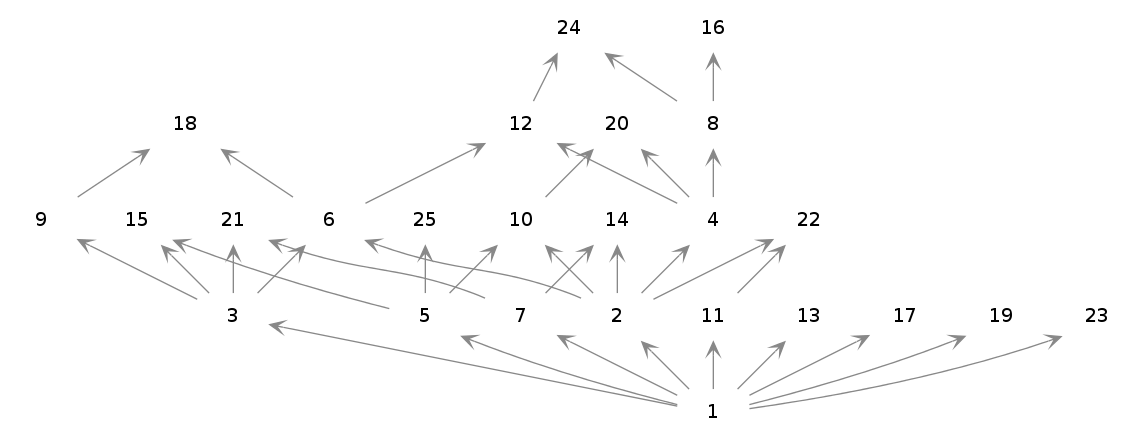
\includegraphics[scale=0.35]{teilbarkeitsordnung.png}
  %% mit dot2tex erzeugt. Aber die Abstände zwischen den Nodes sind viel zu groß.
\begin{tikzpicture}[>=latex',line join=bevel]
%%
\node (24) at (423bp,306bp) [draw,draw=none] {24};
  \node (25) at (315bp,162bp) [draw,draw=none] {25};
  \node (20) at (459bp,234bp) [draw,draw=none] {20};
  \node (21) at (171bp,162bp) [draw,draw=none] {21};
  \node (22) at (603bp,162bp) [draw,draw=none] {22};
  \node (23) at (819bp,90bp) [draw,draw=none] {23};
  \node (1) at (531bp,18bp) [draw,draw=none] {1};
  \node (3) at (171bp,90bp) [draw,draw=none] {3};
  \node (2) at (459bp,90bp) [draw,draw=none] {2};
  \node (5) at (315bp,90bp) [draw,draw=none] {5};
  \node (4) at (531bp,162bp) [draw,draw=none] {4};
  \node (7) at (387bp,90bp) [draw,draw=none] {7};
  \node (6) at (243bp,162bp) [draw,draw=none] {6};
  \node (9) at (27bp,162bp) [draw,draw=none] {9};
  \node (8) at (531bp,234bp) [draw,draw=none] {8};
  \node (11) at (531bp,90bp) [draw,draw=none] {11};
  \node (10) at (387bp,162bp) [draw,draw=none] {10};
  \node (13) at (603bp,90bp) [draw,draw=none] {13};
  \node (12) at (387bp,234bp) [draw,draw=none] {12};
  \node (15) at (99bp,162bp) [draw,draw=none] {15};
  \node (14) at (459bp,162bp) [draw,draw=none] {14};
  \node (17) at (675bp,90bp) [draw,draw=none] {17};
  \node (16) at (531bp,306bp) [draw,draw=none] {16};
  \node (19) at (747bp,90bp) [draw,draw=none] {19};
  \node (18) at (135bp,234bp) [draw,draw=none] {18};
  \definecolor{strokecolor}{rgb}{0.53,0.53,0.53};
  \draw [strokecolor,->] (1) ..controls (580.77bp,42.885bp) and (613.36bp,59.178bp)  .. (17);
  \definecolor{strokecolor}{rgb}{0.53,0.53,0.53};
  \draw [strokecolor,->] (12) ..controls (400.06bp,260.12bp) and (404.82bp,269.63bp)  .. (24);
  \definecolor{strokecolor}{rgb}{0.53,0.53,0.53};
  \draw [strokecolor,->] (3) ..controls (121.23bp,114.88bp) and (88.643bp,131.18bp)  .. (9);
  \definecolor{strokecolor}{rgb}{0.53,0.53,0.53};
  \draw [strokecolor,->] (5) ..controls (341.72bp,116.72bp) and (352.06bp,127.06bp)  .. (10);
  \definecolor{strokecolor}{rgb}{0.53,0.53,0.53};
  \draw [strokecolor,->] (1) ..controls (557.72bp,44.715bp) and (568.06bp,55.056bp)  .. (13);
  \definecolor{strokecolor}{rgb}{0.53,0.53,0.53};
  \draw [strokecolor,->] (6) ..controls (202.06bp,189.29bp) and (185.31bp,200.46bp)  .. (18);
  \definecolor{strokecolor}{rgb}{0.53,0.53,0.53};
  \draw [strokecolor,->] (1) ..controls (504.28bp,44.715bp) and (493.94bp,55.056bp)  .. (2);
  \definecolor{strokecolor}{rgb}{0.53,0.53,0.53};
  \draw [strokecolor,->] (4) ..controls (481.23bp,186.88bp) and (448.64bp,203.18bp)  .. (12);
  \definecolor{strokecolor}{rgb}{0.53,0.53,0.53};
  \draw [strokecolor,->] (9) ..controls (67.939bp,189.29bp) and (84.691bp,200.46bp)  .. (18);
  \definecolor{strokecolor}{rgb}{0.53,0.53,0.53};
  \draw [strokecolor,->] (11) ..controls (557.72bp,116.72bp) and (568.06bp,127.06bp)  .. (22);
  \definecolor{strokecolor}{rgb}{0.53,0.53,0.53};
  \draw [strokecolor,->] (7) ..controls (413.72bp,116.72bp) and (424.06bp,127.06bp)  .. (14);
  \definecolor{strokecolor}{rgb}{0.53,0.53,0.53};
  \draw [strokecolor,->] (2) ..controls (459bp,115.87bp) and (459bp,125.03bp)  .. (14);
  \definecolor{strokecolor}{rgb}{0.53,0.53,0.53};
  \draw [strokecolor,->] (1) ..controls (470.14bp,33.09bp) and (410.39bp,49.26bp)  .. (5);
  \definecolor{strokecolor}{rgb}{0.53,0.53,0.53};
  \draw [strokecolor,->] (2) ..controls (432.28bp,116.72bp) and (421.94bp,127.06bp)  .. (10);
  \definecolor{strokecolor}{rgb}{0.53,0.53,0.53};
  \draw [strokecolor,->] (3) ..controls (144.28bp,116.72bp) and (133.94bp,127.06bp)  .. (15);
  \definecolor{strokecolor}{rgb}{0.53,0.53,0.53};
  \draw [strokecolor,->] (2) ..controls (485.72bp,116.72bp) and (496.06bp,127.06bp)  .. (4);
  \definecolor{strokecolor}{rgb}{0.53,0.53,0.53};
  \draw [strokecolor,->] (2) ..controls (508.77bp,114.88bp) and (541.36bp,131.18bp)  .. (22);
  \definecolor{strokecolor}{rgb}{0.53,0.53,0.53};
  \draw [strokecolor,->] (5) ..controls (315bp,115.87bp) and (315bp,125.03bp)  .. (25);
  \definecolor{strokecolor}{rgb}{0.53,0.53,0.53};
  \draw [strokecolor,->] (10) ..controls (413.72bp,188.72bp) and (424.06bp,199.06bp)  .. (20);
  \definecolor{strokecolor}{rgb}{0.53,0.53,0.53};
  \draw [strokecolor,->] (8) ..controls (531bp,259.87bp) and (531bp,269.03bp)  .. (16);
  \definecolor{strokecolor}{rgb}{0.53,0.53,0.53};
  \draw [strokecolor,->] (6) ..controls (292.77bp,186.88bp) and (325.36bp,203.18bp)  .. (12);
  \definecolor{strokecolor}{rgb}{0.53,0.53,0.53};
  \draw [strokecolor,->] (4) ..controls (504.28bp,188.72bp) and (493.94bp,199.06bp)  .. (20);
  \definecolor{strokecolor}{rgb}{0.53,0.53,0.53};
  \draw [strokecolor,->] (1) ..controls (531bp,43.869bp) and (531bp,53.026bp)  .. (11);
  \definecolor{strokecolor}{rgb}{0.53,0.53,0.53};
  \draw [strokecolor,->] (1) ..controls (603.23bp,27.848bp) and (696.56bp,43.008bp)  .. (23);
  \definecolor{strokecolor}{rgb}{0.53,0.53,0.53};
  \draw [strokecolor,->] (3) ..controls (197.72bp,116.72bp) and (208.06bp,127.06bp)  .. (6);
  \definecolor{strokecolor}{rgb}{0.53,0.53,0.53};
  \draw [strokecolor,->] (4) ..controls (531bp,187.87bp) and (531bp,197.03bp)  .. (8);
  \definecolor{strokecolor}{rgb}{0.53,0.53,0.53};
  \draw [strokecolor,->] (3) ..controls (171bp,115.87bp) and (171bp,125.03bp)  .. (21);
  \definecolor{strokecolor}{rgb}{0.53,0.53,0.53};
  \draw [strokecolor,->] (1) ..controls (591.86bp,33.09bp) and (651.61bp,49.26bp)  .. (19);
  \definecolor{strokecolor}{rgb}{0.53,0.53,0.53};
  \draw [strokecolor,->] (7) ..controls (356.84bp,105.7bp) and (353.88bp,106.93bp)  .. (351bp,108bp) .. controls (292.03bp,129.82bp) and (270.86bp,121.96bp)  .. (21);
  \definecolor{strokecolor}{rgb}{0.53,0.53,0.53};
  \draw [strokecolor,->] (1) ..controls (481.23bp,42.885bp) and (448.64bp,59.178bp)  .. (7);
  \definecolor{strokecolor}{rgb}{0.53,0.53,0.53};
  \draw [strokecolor,->] (8) ..controls (490.06bp,261.29bp) and (473.31bp,272.46bp)  .. (24);
  \definecolor{strokecolor}{rgb}{0.53,0.53,0.53};
  \draw [strokecolor,->] (2) ..controls (428.84bp,105.7bp) and (425.88bp,106.93bp)  .. (423bp,108bp) .. controls (364.03bp,129.82bp) and (342.86bp,121.96bp)  .. (6);
  \definecolor{strokecolor}{rgb}{0.53,0.53,0.53};
  \draw [strokecolor,->] (5) ..controls (254.14bp,105.09bp) and (194.39bp,121.26bp)  .. (15);
  \definecolor{strokecolor}{rgb}{0.53,0.53,0.53};
  \draw [strokecolor,->] (1) ..controls (440.35bp,36.129bp) and (281.29bp,67.941bp)  .. (3);
%
\end{tikzpicture}

  \caption{\label{teilbarkeitsordnung}Die von der Teilbarkeitsordnung auf den
  positiven natürlichen Zahlen induzierte Kategorie (Ausschnitt).}
\end{figure}


\subsection{Zusammenhang mit dem Limesbegriff in der Analysis}

Zum aus der Analysis vertrauten Limesbegriff ist der kategorielle Begriff
insofern verwandt, als dass bei beiden Konzepten die Vorstellung der immer
besser werdenden Approximation tragfähig ist: Die Glieder einer Folge
nähern sich beliebig genau dem Grenzwert an, die Objekte eines filtrierten
Diagramms approximieren immer besser den Kolimes des Diagramms.

Man kann sich aber auch die präzise Frage stellen, ob man den Limes einer reellen
Zahlenfolge tatsächlich als kategoriellen Limes oder Kolimes in einer
geeigneten Kategorie verstehen kann. Die folgende Proposition gibt darauf eine
partielle Antwort:

\begin{prop}Sei~$(x_n)_n$ eine monoton steigende Folge reeller Zahlen. Genau dann
konvergiert diese Folge gegen eine Zahl~$x \in \RR$, wenn das Diagramm
\[ \begin{array}{@{}rcl@{}}
  \NN &\longrightarrow& B\RR \\
  n &\longmapsto& x_n \\
  \text{"`$n \leq m$"'} &\longmapsto& \text{"`$x_n \leq x_m$"'}
\end{array} \]
mit den eindeutigen Morphismen das Objekt~$x \in B\RR$ als Kolimes besitzt.
\end{prop}
Dabei ist mit~$B\RR$ die von der üblichen Ordnung auf~$\RR$ induzierte
Kategorie gemeint. Grenzwerte monoton steigender Folgen lassen sich also
kategoriell als Kolimiten verstehen, und dual lassen sich auch Grenzwerte
monoton fallender Folgen als kategorielle Limiten interpretieren. Für
allgemeine Folgen gibt es aber (wohl) keine solche Übersetzung. Das ist auch
anschaulich plausibel: Den Grenzwert einer monoton steigenden Folge kann man
unter allen reellen Zahlen allein über seine Ordnungsbeziehungen (also kategoriell!) zu
den Folgegliedern charakterisieren, nämlich als ihr Supremum. Für den Grenzwert
einer allgemeinen Folge ist eine solche Charakterisierung dagegen nicht
möglich, stattdessen muss tatsächlich die metrische Struktur beachtet werden.


\subsection{Existenz von Limiten und Kolimiten}

In der Analysis ist die Forderung an eine Folge, zu konvergieren, eine große
Einschränkung: Sogar in vollständigen metrischen Räumen, wie etwa dem der
reellen Zahlen, konvergieren nicht alle Folgen, sondern nur die, die die
Cauchy-Bedingung erfüllen. Metrische Räume, in denen tatsächlich alle Folgen
konvergieren, enthalten zwangsläufig höchstens einen Punkt und sind daher
uninteressant.

Entsprechend ist es ein im Allgemein schwieriges Problem, die Konvergenz oder
Divergenz einer Folge zu entscheiden oder sogar ihren Grenzwert zu berechnen.
In der Kategorientheorie dagegen ist die Situation viel besser [langweiliger?]: Viele
bedeutsame Kategorien enthalten Limiten und Kolimiten \emph{aller} Diagramme
(welche nur eine mengentheoretische Größenbedingung erfüllen müssen).

\begin{defn}Eine Kategorie~$\C$ heißt genau dann \emph{(ko-)vollständig}, wenn
jedes kleine Diagramm in~$\C$ einen (Ko-)Limes besitzt. Dabei heißt ein
Diagramm~$\I \to \C$ genau dann \emph{klein}, wenn seine Indexkategorie~$\I$
klein ist (d.\,h. wenn die Objekt- und Morphismenklassen sogar schon Mengen
bilden).\end{defn}

Etwa ist das archetypische Beispiel einer Kategorie, die der Mengen,
vollständig und kovollständig. Man kann sogar explizit die Limiten und
Kolimiten angeben:

\begin{prop}Die Kategorie der Mengen ist vollständig und kovollständig:
Ist~$F:\I\to\Set$ ein kleines Diagramm, so wird die Menge
\begin{align*}
  \lim F &:= \Bigl\{ (x_i)_{i\in\Ob\I} \in \prod_{i \in \Ob\I} F(i) \ \Big|\
  \text{$F(f)(x_i) = x_j$ für alle~$f:i \to j$ in~$\I$} \Bigr\}
\intertext{vermöge der kanonischen Projektionsabbildungen zu einem Limes
von~$F$ und}
  \colim F &:= \Biggl(\coprod_{i \in \Ob\I} F(i)\Biggr)\Big/{\sim},
\end{align*}
wobei~$({\sim})$ die feinste Äquivalenzrelation mit
\[ \text{für alle $f : i \to j$ in~$\I$, $x \in F(i)$:}\quad
  \langle i, x \rangle \sim \langle j, F(f)(x) \rangle \]
ist, zu einem Kolimes von~$F$.
\end{prop}
\begin{proof}
Die Äquivalenzrelation~$({\sim})$ kann definiert werden als Schnitt über alle
Äqui\-va\-lenz\-re\-la\-tio\-nen auf~$\coprod_{i \in \Ob\I} F(i)$, die die angegebene
Bedingung erfüllen. Dann kann man die Behauptungen nachrechnen.
\end{proof}

Wenn man die Vollständigkeit oder Kovollständigkeit einer Kategorie zeigen
möchte, ist es hilfreich zu wissen, dass sich allgemeine Limiten und Kolimiten
aus gewissen Grundbausteinen zusammenbauen lassen. Folgende Proposition ist
eine aus einer ganzen Reihe ähnlicher Beobachtungen dazu:
\begin{prop}\label{limitengrundbausteine}%
Genau dann enthält eine Kategorie~$\C$ alle endlichen Limiten (d.\,h. Limiten
von Diagrammen mit endlicher Indexkategorie), wenn
\begin{itemize}
\item sie ein terminales Objekt enthält,
\item je zwei Objekte ein Produkt besitzen und
\item je zwei paralelle Morphismen einen Differenzkern besitzen.
\end{itemize}
\end{prop}
Die duale Aussage gilt natürlich ebenfalls: Endliche Kolimiten lassen sich aus
initialen Objekten, Koprodukten und Kodifferenzkernen zusammenbasteln.

\begin{aufg}Zeige in klassischer Logik folgendes bekanntes Resultat von Freyd:
Enthält eine Kategorie tatsächlich \emph{alle} Limiten (nicht nur alle
kleinen), dann wird sie von einer Quasiordnung induziert, d.\,h. je zwei
parallele Morphismen sind gleich. Tipp: Bilde ein über die Menge aller
Morphismen induziertes Produkt.\end{aufg}

\begin{aufg}Beweise Proposition~\ref{limitengrundbausteine}.\end{aufg}


\subsection{Limiten und Kolimiten in Funktorkategorien}

In diesem Abschnitt wollen wir untersuchen, wie Limiten in
Funktorkategorien~$\Funct(\C,\D)$ aussehen. Sei dazu ein Diagramm
$F : \I \longrightarrow \Funct(\C,\D)$
gegeben. Durch "`Nachschaltung der Evaluierungsfunktoren"' erhält man aus
diesem Diagramm für jedes Objekt~$X \in \Ob\C$ jeweils ein Diagramm in~$\D$:
\[ \begin{array}{@{}rrcl@{}}
  F_X : & \I &\longrightarrow& \D \\
  & i &\longmapsto& F(i)(X)
\end{array} \]
Wenn wir voraussetzen, dass all diese Diagramme jeweils einen Limes~$\lim F_X$ in~$\D$
besitzen, können wir (wie in Aufgabe~4 von Übungsblatt~3) einen Funktor
\[ \begin{array}{@{}rrcl@{}}
  L : & \C &\longrightarrow& \D \\
  & X &\longmapsto& \lim F_X
\end{array} \]
basteln. Dann gilt:
\begin{prop}
Der so konstruierte Funktor~$L$ wird (mit welchen Projektionen?) ein Limes des Diagramms~$F$.
\end{prop}
Etwas ungenau kann man diesen Zusammenhang auch über die Formel
\[ (\lim F)(X) = \lim F_X = \lim_i F(i)(X) \]
ausdrücken. Als Motto kann man daher festhalten:
\begin{motto}Besitzt~$\D$ $\I$-förmige Limiten, so werden~$\I$-förmige Limiten
in der Funktorkategorie~$\Funct(\C,\D)$ punktweise berechnet. In diesem Fall
gilt also:
Ein Kegel eines Diagramms~$F : \I \to \Funct(\C,\D)$ ist genau dann ein Limes,
wenn sein Bild unter allen Auswertungsfunktoren~$\ev_X : \Funct(\C,\D) \to \D$,
$X \in \Ob\C$, jeweils ein Limes ist.
\end{motto}


\subsection{Bewahrung von Limiten und Kolimiten}

In der Analysis ist es eine wichtige Frage, ob eine Abbildung~$f$ Limiten
erhält, ob also die Bildfolge einer konvergenten Folge wieder konvergiert, und
zwar gegen das Bild des Grenzwerts. Eine analoge Begriffsbildung gibt es in der
Kategorientheorie:

\begin{defn}Sei~$\I$ eine Indexkategorie. Ein Funktor~$F:\C\to\D$ \emph{erhält
genau dann~$\I$-förmige Limiten}, wenn für jedes Diagramm~$D:\I\to\C$ und jeden
Limes~$K$ dieses Diagramms
\[ \xymatrix{
  & K \ar[ld] \ar[rd] \\
  D(i) \ar[rr] && D(j)
} \]
der Bildkegel unter~$F$
\[ \xymatrix{
  & F(K) \ar[ld] \ar[rd] \\
  F(D(i)) \ar[rr] && F(D(j))
} \]
ein Limes des Diagramms~$F \circ D : \I \to \D$ ist.
\end{defn}

Dabei genügt es nicht, dass das Bild~$F(K)$ der Kegelspitze mit irgendwelchen
neuen Morphismen zu einem Limes von~$F \circ D$ wird. Dual definiert man das
Konzept der Erhaltung von Kolimiten.

\begin{bsp}\label{vectvergiss}%
Der Vergissfunktor~$U : \Vect{\RR} \to \Set$ erhält Produkte, d.\,h.
Limiten der Form $\bullet\ \bullet$. Koprodukte erhält er aber nie: Ist
\[ \xymatrix{
  V \ar[rd] && W \ar[ld] \\
  & V \oplus W
} \]
ein Koproduktdiagramm in der Kategorie der~$\RR$-Vektorräume, so ist das Bild
dieses Diagramms in der Kategorie der Mengen sicher kein Koproduktdiagramm.
Denn die Inklusionsabbildungen~$V \to V \oplus W$, $W \to V \oplus W$ haben
beide das Element~$(0,0)$ in ihrer Wertemenge; die Injektionen in ein
Koprodukt in~$\Set$ hinein haben aber stets disjunktes Bild.
\end{bsp}

\begin{defn}Ein Funktor heißt genau dann \emph{(ko-)stetig}, wenn er alle
kleinen (Ko"~)Li\-mi\-ten, d.\,h. alle~$\I$-förmigen Limiten mit~$\I$ einer kleinen
Indexkategorie, erhält.\end{defn}

In vielen Situationen gibt es einen tieferen Grund, wieso ein Funktor Limiten
oder Kolimiten erhält: Er kann ein sog. rechts- bzw. linksadjungierter Funktor
sein. Das ist etwa beim Vergissfunktor aus dem Beispiel der Fall und erlaubt
ganz ohne explizite Rechnungen als Nachweis sogar die Erhaltung aller Limiten
überhaupt zu folgern.  Wir diskutieren das im Kapitel über adjungierte
Funktoren in Proposition~\ref{limitenbeiadjunktionen}.

\begin{bem}In der Analysis gibt es verschiedene stärke Varianten des bloßen
Konvergenzbegriffs: Etwa kann man die Konvergenzgeschwindigkeit vorgeben.
Auch in der Kategorientheorie gibt es stärkere Limesbegriffe: Etwa ist ein
\emph{absoluter Limes} einer, der unter \emph{allen} Funktoren überhaupt
erhalten bleibt.\end{bem}


\subsubsection{Stetigkeit des Hom-Funktors}

Sei~$A$ ein Objekt einer lokal kleinen Kategorie~$\C$; dann haben wir in
Definition~\ref{defhomfunktor} den kovarianten Hom-Funktor
\[ \Hom_\C(A, \freist) : \C \longrightarrow \Set,\ X \longmapsto \Hom_\C(A,X) \]
eingeführt. Dieser Funktor ist stets stetig:
\begin{prop}Der kovariante Hom-Funktor~$\Hom_\C(A,\freist)$ ist stetig, d.\,h.
für alle kleinen Diagramme~$F : \I \to \C$ mit existierendem Limes ist die
kanonische Abbildung
\[ \lim_i \Hom_\C(A, F(i)) \stackrel{\cong}{\longrightarrow} \Hom_\C(A, \lim_i F(i)) \]
ist bijektiv. Stimmt die Reihenfolge?
\end{prop}


\subsection{Vertauschung von (Ko-)Limiten}

Limiten vertauschen stets mit Limiten, und dual vertauschen Kolimiten stets mit Kolimiten:
\begin{prop}
Sei~$F : \I \times \J \to \C$ ein Diagramm in~$\C$. Sei für jedes Objekt~$i \in
\Ob\I$ jeweils ein Limes~$L_i := \lim_j F(i, \freist)$ gegeben, und sei ferner
ein Limes~$L := \lim_i L_i$ gegeben. Dann ist~$L$ in kanonischer Art und Weise
auch ein Limes~$\lim_{(i,j)} F(i,j)$... genaue Aussage bei nLab nachlesen!
\end{prop}

Allerdings vertauschen im Allgemeinen Limiten nicht mit Kolimiten und
umgekehrt. In einem wichtigen Spezialfall stimmt es aber doch:
\begin{prop}\emph{Filtrierte} Kolimiten vertauschen mit Limiten (nach Set!
genaue Aussage nachlesen).
\end{prop}


\subsection{Kofinale Unterdiagramme}

In der Analysis gibt es folgende Mottos: \emph{Das Weglassen endlich vieler Folgeglieder
ändert nicht das Konvergenzverhalten. Teilfolgen konvergenter Folgen
konvergieren ebenfalls, und zwar gegen denselben Grenzwert.} Analoge Mottos
gibt es auch in der Kategorientheorie; an die Stelle der zur Festlegung einer
Teilfolge~$(a_{n_k})_k$ verwendeten Abbildung~$k \mapsto n_k$ treten
\emph{kofinale Funktoren}:

\begin{defn}
Wir nennen einen Funktor $H : \D_0 \to \D$ genau dann \emph{kofinal}, wenn
für alle Objekte~$d \in \Ob\D$\ldots
\begin{enumerate}
\item[1.] ein Objekt $d_0 \in \Ob\D_0$ und ein Morphismus $d \to
H(d_0)$ in~$\D$ existiert und
\item[2.] für je zwei solcher Morphismen ein Objekt~$\widetilde d_0 \in \Ob\D_0$ und
Morphismen $d_0 \to \widetilde d_0$, $d_0' \to \widetilde d_0$ existieren, deren Bilder
unter~$H$ das Diagramm
\[ \xymatrix{
  d_0 \ar[r] \ar[d] & H(d_0) \ar@{-->}[d] \\
  H(d_0') \ar@{-->}[r] & H(\widetilde d_0)
} \]
kommutieren lassen.
\end{enumerate}
\end{defn}

Etwa ist der Inklusionsfunktor~$B (2\NN) \to B(\NN)$ kofinal, wenn~$\NN$ die
Menge der natürlichen Zahlen mit ihrer gewöhnlichen Ordnung und~$2\NN$ die
Teilordnung der geraden Zahlen bezeichnet.

\begin{prop}
Sei~$H : \D_0 \to \D$ ein kofinaler Funktor und~$F : \D \to \C$
ein~$\D$-förmiges Diagramm in einer Kategorie~$\C$. Dann gilt:
\begin{enumerate}
\item Die Kategorie der Kokegel von~$F$ ist äquivalent zur Kategorie der
Kokegel von~$F \circ H$.
\item Die Angabe eines Kolimes von~$F$ ist gleichwertig mit der Angabe eines
Kolimes von~$F \circ H$.
\end{enumerate}
\end{prop}
\begin{proof}
Der erste Teil ist Gegenstand von Aufgabe~4 von Übungsblatt 5. Die zweite
Aussage folgt sofort aus dem ersten, da ja ein Kolimes von~$F$ bzw.~$F \circ H$
als initiales Objekt in der entsprechenden Kokegelkategorie definiert ist.
\end{proof}

Natürlich gilt die duale Aussage für Limiten: Ist in der Situation der
Proposition der Funktor~$H$ aufgefasst als Funktor~$\D_0^\op \to \D^\op$
kofinal, so ist die Angabe eines Limes von~$F$ gleichwertig mit der Angabe
eines Limes von~$F \circ H$.

\begin{bsp}Wir haben die~$p$-adischen Ganzzahlen als Limes des Diagramms
\[ \cdots \lra \ZZ/(p^2) \lra \ZZ/(p^1) \lra \ZZ/(p^0) \]
definiert. Genauso gut, wenn auch ein wenig willkürlich, hätten wir sie als
Limes des Diagramms
\[ \cdots \lra \ZZ/(p^5) \lra \ZZ/(p^4) \lra \ZZ/(p^3) \]
definieren können.\end{bsp}

% XXX: Der Kapitelname ist schlecht. Müssen nämlich nicht wirklich Unterdiagramme sein!

% Hom linksexakt

% Rechenregel Hom
